\chapter{Preliminaries
\label{ch:preliminaries}}
In this section we will discuss the basic problem we're trying to solve.  
As this problem is generally computationally intractable, approximate solutions 
must be tried, and we will review those in Section~\ref{sec:approx_methods}. 
For certain special cases the exact solution is in fact available, and 
these constitute a valuable check on our approximations. We use one such 
special system, the one dimensional Hubbard model, in this work, and will 
briefly describe the model in \ref{sec:hubbard_hamiltonian}.

\section{The electronic structure problem}
\label{sec:motivation}
The goal of quantum chemistry is to simulate and predict the behavior 
of chemical systems. At the root of chemical phenomena is the motion 
of electrons in the field of the nuclei. Together, electrons form a quantum 
many-body system. If one could efficiently simulate the energy and 
the state of this system numerically, many questions of chemistry could be 
answered.

Since the advent of quantum mechanics all ingredients of many-body simulations 
are known. One needs to find the eigenvectors and eigenvalues of the 
Hamiltonian describing the system:
%
\begin{equation}
 \hat{H} | \Psi \rangle = E | \Psi \rangle
 \label{eq:schroedinger}
\end{equation}
%
where $\Psi(\vec{x_{1}}, \vec{x_{2}}, \vec{x_{3}}\ldots 
\vec{x_{M}}) = \langle \vec{x}_{1}, \vec{x}_{2}, \vec{x}_{2}, \ldots |\Psi 
\rangle$ is a wavefunction describing the state of an $M$-electron system 
and $E$ is the energy of the state. The variables $\vec{x}$ describe the 
degrees of freedom of the electrons, like coordinates and spin.
The Hamiltonian is usually written in a short form, due to the 
equivalence of quantum particles:
%
\begin{equation}
\begin{aligned}
 \hat{H} = h^{0} + \sum_{n} \hat{h}(\vec{x^{\star}_{n}}, \vec{x}_{n}) + 
\frac{1}{2} \sum_{n \neq m} \hat{V}(\vec{x^{\star}_{m}}, \vec{x^{\star}_{n}}, 
\vec{x}_{m}, 
\vec{x}_{n}) 
\end{aligned}
\end{equation}
%
Here $h^{0}$ is a constant, $\hat{h}$ is a one-body part, e.g. it acts on each 
electron individually, and $\hat{V}$ is a two body part, acting on every pair 
of electrons. 

To solve~\ref{eq:schroedinger} in practice a discrete basis with $N$ 
functions is introduced for each of the variables $\vec{x}$, the procedure 
mathematicians would call Galerkin discretization. We denote these new 
$N$-valued discrete spaces by $\mathcal{V}$. As the number of basis functions 
increases, the solution of the discretized problem will approach the true 
solution of~\ref{eq:schroedinger}. After standard approximations, like the 
Born-Oppenheimer approximation,~\cite{jensen2017introduction} the molecular 
Hamiltonian becomes:
%
\begin{equation}
 \hat{H} = h^{nr} + h_{\mu \nu} a^{\dagger}_{\mu} a_{\nu} + \frac{1}{2} V_{\mu 
\nu \lambda \sigma} a^{\dagger}_{\mu} a^{\dagger}_{\nu} a_{\sigma} a_{\lambda}
\label{eq:hamiltonian}
\end{equation}
%
We imply summation over repeated indices in the expression above and the rest 
of the text unless otherwise stated. In Eqn.~\ref{eq:hamiltonian} the constant 
$h^{nr}$ is the nuclear repulsion energy, the one-body part $h$ describes the 
kinetic energy of an electron and its attraction to the nuclei:
%
\begin{equation}
 h_{\mu \nu} = \int d\vec{x_{1}} ~ \mu^{\star}(\vec{x_{1}}) \left( - 
\frac{1}{2} \nabla^2 - \sum_{a} \frac{Z_{a}}{|\vec{x_{1}} - 
\vec{r_{a}}|} \right) \nu(\vec{x_{1}})
\end{equation}
% 
The functions $\mu(\vec{x}), \nu(\vec{x})$ are basis functions used for the 
discretization of the problem and $r_{a}$ and $Z_{a}$ are the 
position and the charge of the nuclei. The two-body, or electron repulsion 
part, is
%
\begin{equation}
 V_{\mu \nu \lambda \sigma} = \int \int d\vec{x_{1}} d\vec{x_{2}}~ 
\mu^{\star}(\vec{x_{1}}) \nu^{\star}(\vec{x_{2}}) 
\frac{1}{|\vec{x_{1}} - \vec{x_{2}}|} 
\sigma(\vec{x_{2}}) \lambda(\vec{x_{1}}) 
\end{equation}
% 
We denoted by $a^{\dagger}_{\mu}$ and $a_{\mu}$ creation and 
annihilation operators. For example, $a^{\dagger}_{\mu}$ creates a single 
particle state $a^{\dagger}_{\mu} | - \rangle = | \mu \rangle$, where $| - 
\rangle$ is the physical vacuum. Equivalently, $a^{\dagger}_{\mu}$ and 
$a_{\mu}$ can be thought as simply the $\mu$-th unit vector (or its adjoint) in 
the discrete space $\mathcal{V}$, and $| - \rangle$  as a zero vector.

Despite the simple structure of the Hamiltonian, even a discretized
Schr{\"o}dinger equation is hard to solve. The solution is contained in an 
antisymmetric product (due to the Pauli exclusion 
principle) of single particle vector spaces. The resulting space, called 
the Hilbert space of the problem, is: 
%
\begin{equation}
 \mathcal{H} = \underbrace{\mathcal{V} \times \mathcal{V} \times \mathcal{V} 
\times \ldots}_{M ~\mathrm{times}}
\end{equation}
%
The Hamiltonian is thus a matrix in $\mathcal{H} \times \mathcal{H}$. The total 
size of the eigenvector of the Hamiltonian $|\Psi \rangle$ is 
on the order of $N^{M}$ (it is actually $N \choose M$ because $\mathcal{H}$ is 
an antisymmetric vector space). Even for relatively small $M$ and $N$ a direct 
calculation of $|\Psi \rangle$ becomes prohibitive. The main problem of 
theoretical chemistry is how to build feasible and accurate 
approximations to the true eigenvectors of $H$.

A commonly used approach is to use the variational 
principle~\cite{jensen2017introduction} to 
calculate the energy expectation value $\tilde{E}$ of a test wavefunction 
$\tilde{\Psi}$:
%
\begin{equation}
 \tilde{E} = \frac{\langle \tilde{\Psi} | H | \tilde{\Psi} \rangle}{\langle 
\tilde{\Psi} |\tilde{\Psi} \rangle} 
\end{equation}
%
It can be proven~\cite{levine2000quantum} that this expectation value for a 
normalizable function is an upper bound of the exact energy:
%
\begin{equation}
 E \geq E_{\mathrm{exact}}
\end{equation}
Although not all approaches to solve \ref{eq:schroedinger} are variational, 
variational nature is a valuable property of any particular method. 

\section{Solving the Schr{\"o}dinger equation}
\label{sec:solving}
\subsection{Exact solution}
As we mentioned before, the direct solution of the Sch{\"o}dinger equation is 
hard to obtain. One may still, however, embark on this task for very small 
systems. Let us introduce a basis of all states with $M$ electrons in the 
Hilbert space $\mathcal{H}$. This basis will contain all possible products of 
$M$ creation operators. Due to the antisymmetry of the 
wavefunction for electrons:
%
\begin{equation}
  \Psi(\vec{x_{1}}, \vec{x_{2}}) = - \Psi(\vec{x_{2}}, \vec{x_{1}}) 
\end{equation}
%
those products will contain only the combinations of $a^{\dagger}_{\mu}$ 
without repetitions over the index $\mu$ (a repeated index will necessarily 
turn the product to zero):
%
\begin{equation}
 | \phi \rangle = \prod_{k=1}^{M} a^{\dagger}_{\mu_{k}} |- \rangle  
 \label{eq:slater_determinant}
\end{equation}
%
In total there will be $N \choose M$ products of the
form~\ref{eq:slater_determinant}, usually called Slater determinants or 
configurations. The Hamiltonian matrix can be written in this basis and 
diagonalized:
%
\begin{equation}
\begin{aligned}
 H_{ij} &= \langle \phi_{i} | \hat{H} | \phi_{j} \rangle \\
 | \Psi_{i} \rangle &= U_{ij} |\phi_{j} \rangle
\end{aligned}
\end{equation}
%
The eigenvectors $| \Psi \rangle$ obtained in this way and their respective 
eigenvalues are exact solutions to the Schr{\"o}dinger equation in a given 
basis. When available, they are often used as reference values in the
evaluation of the quality of quantum chemistry algorithms. Direct 
diagonalization, however, is possible only for the smallest systems. The 
simulation of a 12-electron system, such as two carbon atoms, in a mediocre 
basis set of 10 basis functions per electron will involve diagonalization of 
a matrix of size $1.054 \cdot 10^{16}$ which is already at the border of 
today's computational capabilities.

One may notice, however, that the molecular Hamiltonian is almost diagonal in 
the $M$-particle Hilbert space, as only one- and two-body parts are non-zero. 
This provides grounds for an important approximate method we are going to 
consider next. 

\subsection{Hartree-Fock solution}
The Hartree-Fock (HF) method is the starting point of most many-body approaches.
The idea of Hartree-Fock is to find a single best determinant to 
approximate the wavefunction:
%
\begin{equation}
 |\Psi_{SD} \rangle = \prod_{k=1}^{M} c_k^{\dagger} | -\rangle, \qquad 
c_{k}^{\dagger} = C_{\mu k} \cdot a^{\dagger}_{\mu}
\label{eq:single_determinant}
\end{equation}
% 
The parameters of this \emph{ansatz} are contained in the basis transformation 
matrix $C$. The energy 
of the state~\ref{eq:single_determinant} is:
%
\begin{equation}
 E = \frac{\langle \Psi_{SD} | H | \Psi_{SD} \rangle}{\langle \Psi_{SD} | 
\Psi_{SD} \rangle}
 \label{eq:hf_energy}
\end{equation}
%
The solution is found by minimizing the energy in~\ref{eq:hf_energy}, 
while constraining matrix $C$ to be unitary. The later is equivalent to 
minimizing a Lagrangian:
%
\begin{equation}
\begin{aligned}
L(C, \epsilon) = h_{\mu \nu} \rho_{\nu \mu} &+ \frac{1}{2} 
V_{\mu \lambda \nu \sigma} \rho_{\nu \mu } \rho_{\sigma \lambda}  + 
\epsilon_{ij}(C^{\ast}_{\mu i} S_{\mu \nu} C_{\nu j} - 1_{N \times N})\\
\rho_{\nu \mu} &= C^{\ast}_{\mu i} C_{\nu i} 
\label{eq:hf_lagrangian}
\end{aligned}
\end{equation}
%
Here $C$ is the basis transformation one is solving for, $\epsilon$ is a 
set of Lagrange multipliers used to enforce the unitary constraint, $1_{N 
\times N}$ is the identity matrix and $S_{\mu \nu} = \langle a^{\dagger}_{\mu} 
a_{\nu} \rangle $ is an overlap matrix of the possibly non-orthogonal original 
basis vectors $a$. Let us note that the Hartree-Fock method 
is variational, and hence provides an upper bound for
the energy.\cite{levine2000quantum} 

There are multiple ways of solving the Hartree-Fock equations, which we will 
not discuss here, but rather present a final result of the most well-known 
method of Roothaan.~\cite{roothaan1951new} By taking the derivative 
of~\ref{eq:hf_lagrangian} with respect to $C$, one ends up with a matrix 
equation:
%
\begin{equation}
\begin{aligned}
 FC^{\ast} &=  C^{\ast} S \epsilon\\
 F_{\mu \nu} &= h_{\mu \nu} + V_{\mu \lambda \nu \sigma} \rho_{\sigma \lambda} 
 \label{eq:hf_roothaan}
\end{aligned}
\end{equation}
%
Equation~\ref{eq:hf_roothaan}, which looks like an eigenvalue problem for 
the Fock matrix $F$, is non-linear in $C$. It is solved by iteration starting 
from a guess for the transformation $C$. At convergence the matrix $C$ presents 
a transformation from the atomic orbital (AO) to molecular orbital (MO) basis. 
The Fock matrix in the MO basis is diagonal, and its diagonal elements can be 
interpreted as single particle energy levels. 

Roothaan's equation amounts to an important interpretation of the 
Hartree-Fock method. Note that if there would be no interaction term in the 
Hamiltonian, the Hartree-Fock would correspond to the exact 
diagonalization, and a Slater determinant, which is an antisymmetric direct 
product of single particle wavefunctions, would be an exact 
eigenstate. The Fock matrix in Eqn.~\ref{eq:hf_roothaan}, thus is a diagonal
approximation of the Hamiltonian, where the actual two-particle interaction 
$\hat{V}$ is replaced by a one-body term $\hat{V}_{eff} = \hat{V} \hat{\rho}$. 
The HF solution describes the electrons as if they would not immediately repel 
each other through Coulombic interaction, but rather move 
independently in an average potential $\hat{V}_{eff}$ of all other electrons. 
In reality, however, the electrons avoid each other dynamically. This brings us 
to the concept of electronic correlation: the true solution would need to 
account for the correlated motion of electrons. We will discuss this in more 
detail in the next section.

Overall, the Hartree-Fock method is a cornerstone of quantum chemistry due to 
its simplicity and theoretical basis. The computational cost of Hartree-Fock is 
$O(N^4)$ floating point operations in its simplest variants (and much less 
in optimized formulations\cite{goedecker1999linear}), which makes it one of the 
most affordable methods in electronic structure theory. Despite not being 
widely used on its own in practical simulations, it remains a usual starting 
point of most many-body approaches.


\subsection{Electronic correlation
\label{sec:electronic_correlation}}

Put simply, electronic correlation is the difference between the exact and 
Hartree-Fock solution, and the correlation energy is the difference between 
the HF and exact energies. We will classify correlation based on two 
sources of errors introduced by the Hartree-Fock method; however, this division 
is only relative:

\begin{itemize}
\item Dynamic or weak correlation arises from small deviations of 
the Hartree-Fock potential from the faithful two-body interaction. It can be 
interpreted as an effect of short-range instantaneous repulsion between 
electrons.
\item Static or strong correlation emerges when the Hartree-Fock potential 
significantly deviates from the real two-body interaction, e.g. when the 
Hamiltonian is not a diagonally dominant matrix. Static correlation 
manifests as a near or exact degeneracy of different Slater determinants, and 
the single determinant picture becomes incorrect.
\end{itemize}

Let us illustrate the regions where different types of error of the HF method 
dominate in the process of nitrogen dissociation. 
%
\begin{figure}[tb]
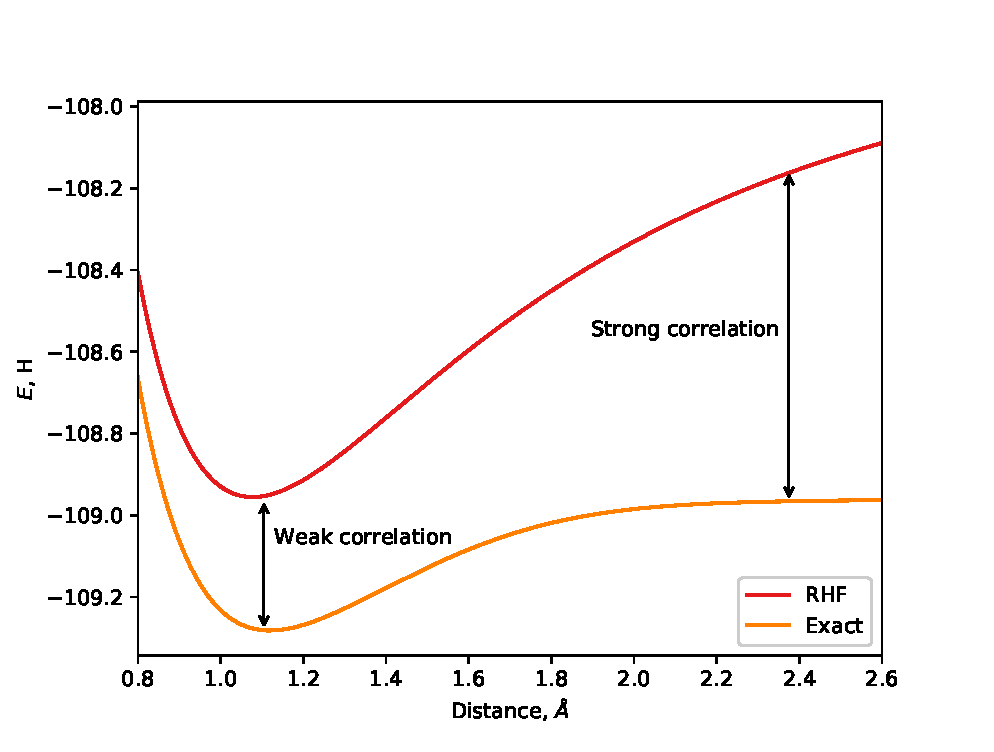
\includegraphics[width=\columnwidth]{figures/prelim/hf_exact}
\caption{Regions of weak and strong correlation along the dissociation 
curve of the nitrogen molecule. RHF refers to restricted Hartree-Fock, exact is 
taken from the exact diagonalization data.
\label{fig:n2_hf_exact}}
\end{figure}
%
Near equilibrium the difference of Hartree-Fock and and exact energies is 
mostly related to short-range dynamical electronic repulsion. When the 
bond is stretched, the bonding, $\sigma^{\ast}_{2p}$ and $\pi_{2p}$ 
orbitals become degenerate, as well as antibonding $\sigma^{\ast}_{2p}$ and 
$\pi_{2p}$ orbitals. Finally, at infinite distance all $2p$ orbitals are the 
same, which leads to the major overestimation of dissociation energy by the HF 
method. Let us now provide some examples of different types of correlation and 
its relation to physical phenomena.

Most correlation in "normal" systems is dynamical. Typical examples 
are usual organic molecules at equilibrium, most metals, semiconductors 
etc. While HF accounts for around $99\%$ of electronic energy, proper 
description of dynamical correlation is crucial in quantitative calculations.
For example, even for atoms, HF excitation energies may be wrong by 
more than $40\%$~\cite{wilson2013methods}, which leads to incorrect prediction 
of ionization potentials. The lack of correlation leads to too short bonds at 
equilibrium, incorrect bond angles, errors in the dipole moments and too high 
harmonic vibrational frequencies.~\cite{helgaker2014molecular, 
scott1996harmonic} HF usually predicts too high reaction barriers, which can be 
understood by the inability of HF to describe stretched bonds. Finally, the 
Hartree-Fock approach is unable to predict pure dispersion 
interaction, correlation bound anions~\cite{voora2013existence} and similar 
systems.

Statically correlated systems are where the shortcomings of Hartree-Fock theory 
are most pronounced, as the independent particle picture becomes inappropriate. 
Static correlation is very common in extended systems and materials 
where $d$- and $f$-electron shells of atoms interact. Among many phenomena 
caused by strong correlation are large resistivity changes, huge volume changes 
across phase transitions, heavy fermion behavior, large 
magnetoresistence and high temperature superconductivity.~\cite{imada1998metal, 
kotliar2004strongly}. Strongly correlated systems are of great importance and 
constant theoretical interest. Accounting for strong correlation is challenging 
for modern electronic structure methods.

As we hope the reader is convinced, the proper description of electronic 
correlation is essential for quantitative many-body simulations. We should now 
follow with the discussion of the approximate many-body methods.

\section{Approximate many-body methods
\label{sec:approx_methods}}
\subsection{Configuration expansion}
As an exact solution of the Schr{\"o}dinger equation can be obtained by 
diagonalizing the Hamiltonian in the basis of all possible determinants, one 
may try to do it over a subset of configurations to save on numerical cost. 
On the other hand, the HF solution $|\Phi_{0}\rangle$ is the best single 
determinant representation of the wavefunction. A natural idea is then to build 
a subset of configurations which are close to $|\Psi_{0}\rangle$:
%
\begin{equation}
\begin{aligned}
 |\Psi \rangle &= u_{0} |\Psi_{0}\rangle + u_{i}^{a} 
c^{\dagger}_{a} c_{i} |\Psi_{0}\rangle + u_{ij}^{ab} c^{\dagger}_{a} 
c^{\dagger}_{b} c_{j} c_{i} |\Psi_{0}\rangle + u_{ijk}^{abc} 
c^{\dagger}_{a} c^{\dagger}_{b} c^{\dagger}_{c} c_{k} c_{j} c_{i} 
|\Psi_{0}\rangle + \ldots \\
 &= \hat{U}_{0} |\Psi_{0}\rangle + \hat{U}_{1} |\Psi_{0}\rangle + \hat{U}_{2} 
|\Psi_{0}\rangle + \hat{U}_{3} 
|\Psi_{0}\rangle \ldots
\end{aligned}
\label{eq:ci_expansion}
\end{equation}
%
Here expansion coefficients $u$ are used for the different orders of 
substituted determinants. We denote occupied HF states by indices 
$i,j,k,\ldots$ and unocupied states by $a,b,c,\ldots$. Note that because 
operators $c$ act in an orthogonal HF basis, all of the terms 
in~\ref{eq:ci_expansion} represent orthogonal configurations. 
Expansion~\ref{eq:ci_expansion} is the basis of many traditional many body 
methods, the simplest example being the Configuration Interaction (CI) method. 
By taking the expectation value of the Hamiltonian with $|\Psi\rangle$ 
and applying the linear variational theorem one ends up with an eigenvalue 
problem for the coefficients $U$:
%
\begin{equation}
 HU = EU
 \label{eq:ci_eigenvalue}
\end{equation}
%
The solution to the above equation provides a variational estimate of 
the energy. It is evident that when all substitutions in $|\Phi_{0}\rangle$ are 
taken we would return to the exact diagonalization, or the full 
configuration interaction (FCI) problem. To make the computation affordable,the 
expansion~\ref{eq:ci_expansion} is usually truncated at double excitations:
%
\begin{equation}
 |\Psi \rangle = u_{0} |\Psi_{0}\rangle + u_{i}^{a} 
c^{\dagger}_{a} c_{i} |\Psi_{0}\rangle + u_{ij}^{ab} c^{\dagger}_{a} 
c^{\dagger}_{b} c_{j} c_{i} |\Psi_{0}\rangle
\end{equation}
%
Truncated CI methods are not very popular in modern calculations. 
Nevertheless, they are used sometimes if excited states are of interest 
and excitation energies need to be 
calculated.~\cite{sherrill1999configuration,head1994doubles}
The problem with the truncated CI approach is that it is neither size 
consistent nor size extensive.~\cite{helgaker2014molecular, 
jensen2017introduction} 

A method is size consistent~\cite{pople1976theoretical} if the energy of two 
non-interacting fragments $A$ and $B$ is the sum of the energies of those 
fragments calculated independently
\begin{equation}
 E(A \overset{d \longrightarrow \infty}{-} B) = E(A) + E(B)
\end{equation}

Size extensivity means that the energy scales linearly with the size of the 
system. For example, the energy of $k$ interacting fragments, such as Helium 
atoms far apart from each other, should equal to the sum of energies of 
individual fragments.
\begin{equation}
 E(k \cdot \mathrm{He}) = k \cdot E(\mathrm{He})
\end{equation}
In thermodynamics extensive quantities scale with the system 
size,~\cite{bartlett1978many} therefore size extensivity is a desirable 
property of any many-body approach.

It turns out that there is a better way of parameterizing the wavefunction in 
the form~\ref{eq:ci_expansion}, which eliminates the drawbacks of CI. This way 
is provided by the coupled cluster ansatz.

\subsection{Coupled Cluster theory}
Since its introduction in nuclear physics,\cite{coester1958bound, 
coester1960short} coupled cluster has become highly popular in quantum 
chemistry due to its exceptional ability to capture weak electronic 
correlation, while still having polynomial computational cost in the size of 
the basis. Another attractive property of CC theory is that while having the 
same number of parameters as CI methods, CC methods are size consistent and 
size extensive\footnote{Coupled cluster is size 
extensive and size consistent only when the reference 
wavefunction has these properties. For example, 
restricted HF-based coupled cluster is not extensive nor consistent in a case 
when an even number of electrons is split into two fragments with an odd number 
of electrons.}, \cite{pople1978electron, 
bartlett1978many, crawford2000introduction, bartlett2007coupled}. In coupled 
cluster the wavefunction is parameterized with an exponential ansatz:
%
\begin{equation}
 |\Psi\rangle = e^{\hat{T}} |\Psi_{0}\rangle
 \label{eq:cc_ansatz}
\end{equation}
Here the excitation operator $\hat{T}$ acts on a reference wavefunction 
$|\Psi_{0}\rangle$ (usually a Hartree-Fock determinant). The excitation 
operator has the same form as in case of CI:
%
\begin{equation}
\begin{aligned}
 \hat{T} &= {}^1\hat{T} + {}^2\hat{T} + {}^3\hat{T} + \ldots \\ 
 &= {}^{1}T_{i}^{a} c^{\dagger}_{a} c_{i} + \frac{1}{4} {}^2T_{ij}^{ab} 
c^{\dagger}_{a} c^{\dagger}_{b} c_{j} c_{i} + \frac{1}{36} {}^3T_{ijk}^{ab} 
c^{\dagger}_{a} c^{\dagger}_{b} c^{\dagger}_{c} c_{k} c_{j} c_{i} 
+\ldots
\end{aligned}
\end{equation}
The coefficient tensors $T$ are called cluster amplitudes. An excitation 
operator of order $n$ is defined by the following expression:
%
\begin{equation}
 {}^{n}\hat{T} = \frac{1}{(n!)^2}{}^{n}T_{ijk\ldots}^{abc\ldots} 
c^{\dagger}_{a} c^{\dagger}_{b} c^{\dagger}_{c} \ldots c_{k} c_{j} 
c_{i} 
\end{equation}
%
The exponential of the excitation operator is understood in terms of a 
polynomial series. Note that in contrast with CI, this ansatz contains not only 
linear excitations, but also products of excitations:
%
\begin{equation}
\begin{aligned}
  & e^{\hat{T}} |\Psi_{0}\rangle = \\
  & (1 + \hat{T} + \frac{1}{2} \hat{T}^{2} + \frac{1}{6} \hat{T}^3 + \ldots) | 
\Psi_{0} \rangle = \\
  & (1 + {}^{1}\hat{T} + \frac{1}{2}({}^{1}\hat{T})^{2} + \ldots + \\
  & {}^{2}\hat{T} + \frac{1}{2}({}^{2}\hat{T})^{2} + \ldots + \\
  & ({}^{1}\hat{T}) ({}^{2}\hat{T}) + \frac{1}{2}({}^{1}\hat{T})^{2} 
({}^{2}\hat{T}) + \ldots) |\Psi_{0} \rangle \\
\end{aligned}
\end{equation}
%
The size extensivity of coupled cluster is a direct consequence of the 
product terms occuring in the exponential function. 

The energy expression can be obtained by inserting~\ref{eq:cc_ansatz} into the 
Schr{\"o}dinger equation:
%
\begin{equation}
 \hat{H} e^{\hat{T}} | \Psi_{0} \rangle  = E |\Psi_{0} \rangle
 \label{eq:half_cc_schroedinger}
\end{equation}
%
This equation, however, can not be solved variationally with low 
cost. The expectation value would be:
%
\begin{equation}
 \frac{\langle \Psi_{0} | e^{\hat{T}^{\dagger}} \hat{H} e^{\hat{T}} | \Psi_{0} 
\rangle}{\langle \Psi_{0} | e^{\hat{T}^{\dagger}} e^{\hat{T}} |\Psi_{0} 
\rangle} = E 
\end{equation}
%
The variational expression above contains all possible excitations up to the 
number of electrons $M$ and no natural truncation scheme exists. 
Solving~\ref{eq:half_cc_schroedinger} variationally thus may not be easier 
than solving the FCI problem. Alternatively, 
Equation~\ref{eq:half_cc_schroedinger} can be solved projectively by 
multiplying it from the left by $e^{-\hat{T}}$:
%
\begin{equation}
 e^{-\hat{T}} \hat{H} e^{\hat{T}} |\Psi_{0} \rangle = E | \Psi_{0} \rangle
\end{equation}
%
The similarity transformed Hamiltonian $\bar{H} = e^{-\hat{T}} \hat{H} 
e^{\hat{T}}$ can be significantly simplified by using 
the Baker-Campbell-Hausdorf (BCH) expansion~\cite{crawford2000introduction, 
shavitt2009many}, which leads 
to nested commutators of the amplitudes and the Hamiltonian:
%
\begin{equation}
\begin{aligned}
  &e^{-\hat{T}} \hat{H} e^{\hat{T}} = \hat{H} + \left[ \hat{H}, \hat{T} \right] 
+ \frac{1}{2!} \left[ \left[ \hat{H}, \hat{T} \right], \hat{T} \right] +\\
&\frac{1}{3!} \left[ \left[ \left[  \hat{H}, \hat{T} \right], \hat{T} \right], 
\hat{T} \right] + \frac{1}{4!} \left[ \left[ \left[ \left[ \hat{H}, \hat{T} 
\right], \hat{T} \right], \hat{T} \right], \hat{T} \right] + \ldots
\end{aligned}
\label{eq:bch_expansion}
\end{equation}
%
Here $\left[ \hat{H}, \hat{T} \right] = \hat{H} \hat{T} - \hat{T}\hat{H}$.
To evaluate the BCH expansion one needs to start with the Hamiltonian in the 
HF basis. The transformation of the Hamiltonian to the mean field basis can 
be done by using operator algebra (see, for example 
Ref.~\cite{crawford2000introduction} for a complete derivation of this 
expression):
%
\begin{equation}
 \hat{H} = E_{0} + F_{q}^{p} c^{\dagger}_{p} c_{q} + \frac{1}{4} (V_{rs}^{pq} 
- V_{sr}^{pq}) c^{\dagger}_{p} c^{\dagger}_{q} c_{r} c_{s}
\end{equation}
%
Here $E_{0}$ is the Hartree-Fock energy, $F$ is a Fock matrix 
(see~\ref{eq:hf_roothaan}), and $V$ is the two electron interaction in the 
molecular orbital basis. The indices $p,q,r,s,\ldots$ in the Hamiltonian are 
general indices, e.g. they run over both occupied and virtual spaces.

By using the commutator arithmetic~\cite{shavitt2009many} it can be shown that 
each commutator between $\hat{H}$ and $\hat{T}$ transforms one general index 
of the Hamiltonian into a Kronecker delta function. As the Hamiltonian has only 
four different general operators, there can only be four commutators with 
$\hat{T}$, and the BCH expansion naturally truncates after the fifth term in 
Eqn.~\ref{eq:bch_expansion}. The similarity transformed Hamiltonian $\bar{H}$ 
will thus be a polynomial of up to fourth order in excitation operators 
$\hat{T}$.

If the excitation operator $\hat{T}$ contained all possible orders of 
excitations~$\{ {}^{1}\hat{T}, {}^{2}\hat{T}, \ldots \}$, 
the coupled cluster would be equivalent to exact diagonalization. To have a 
practical method one needs to truncate $\hat{T}$. The most common 
truncation level is doubles, e.g:
%
\begin{equation}
 \hat{T} =  {}^{1}T_{i}^{a} c^{\dagger}_{a} c_{i} + \frac{1}{4} {}^2T_{ij}^{ab} 
c^{\dagger}_{a} c^{\dagger}_{b} c_{j} c_{i}
\end{equation}
%
The order of excitation operator $\hat{T}$ determines the name of a particular 
coupled cluster method, with \textbf{S} meaning singles, \textbf{D} denoting 
doubles, \textbf{T} referring to triples etc. Note that by construction CCSD is 
exact for 2-electron systems, CCSDT is exact for 3-electron systems and so on. 
The effect of including single excitations on the accuracy of coupled cluster 
is usually not large, and hence they can often be omitted resulting in the 
simpler coupled cluster with doubles (CCD) method. The cost of coupled cluster 
rises quickly with the order of excitation operator, being of order $O(N^6)$ 
for CCSD, $O(N^8)$ for CCSDT and $O(N^{10})$ for CCSDTQ (see 
chapter~\ref{ch:tcc} for a detailed discussion).

After using the BCH expansion, we are finally in a position to formulate a 
general coupled cluster method. The similarity transformed Schr{\"o}dinger 
equation is:
%
\begin{equation}
 e^{-\hat{T}} \hat{H} e^{\hat{T}} |\Psi_{0}\rangle = E |\Psi_{0}\rangle
 \label{eq:sim_cc_schroedinger}
\end{equation}
It is obvious that the energy can be extracted by taking an expectation value 
with $\langle \Psi_{0}|$. The energy equation is:
%
\begin{equation}
 E = \langle \Psi_{0} | \bar{H} | \Psi_{0} \rangle
 \label{eq:cc_energy}
\end{equation}
The energy expression contains only single (if present in the excitation 
operator $\hat{T}$) and double excitations. Higher orders of 
excitation operator can not be compensated by the Hamiltonian, and would 
necessarily produce orthogonal configurations on the left and right hand sides 
of the expectation value in~\ref{eq:cc_energy}. By using these Slater-Condon 
rules~\cite{jensen2017introduction} the energy of coupled cluster is:
%
\begin{equation}
\begin{aligned}
 E &= \langle \Psi_{0} | (1 - {}^{1}\hat{T} - {}^{2}\hat{T} + \ldots) H (1 + 
{}^{1}\hat{T} + \frac{1}{2} ({}^{1}\hat{T})^2 + \ldots + {}^2 \hat{T} + \ldots) 
= \\
& \langle \Psi_{0} | \hat{H} | \Psi_{0} \rangle + \langle \Psi_{0} | \hat{H} 
({}^{1}\hat{T})| 
\Psi_{0} \rangle + \frac{1}{2} \langle \Psi_{0} | \hat{H} ({}^{1}\hat{T})^2 | 
\Psi_{0} 
\rangle + \langle \Psi_{0} | \hat{H} ({}^{2} \hat{T})| \Psi_{0} \rangle
\end{aligned}
\end{equation}
%
The energy expression justifies the usual truncation of the cluster operator 
$\hat{T}$ at doubles. To have a working theory, however, one would need to 
determine cluster amplitudes $\{{}^{1}T, {}^{2}T, {}^{3}T, \ldots$. This can be 
done by projecting the similarity transformed Hamiltonian onto a set of excited 
configurations $\{ \langle \Psi_{i}^{a}, \Psi_{ij}^{ab}, \Psi_{ijk}^{abc}, 
\ldots \}$: 
%
\begin{equation}
\begin{aligned}
 \langle{\Psi_{i}^{a}} | \bar{H} | \Psi_{0} \rangle = 0 \\
 \langle{\Psi_{ij}^{ab}} | \bar{H} | \Psi_{0} \rangle = 0  \\
 \langle{\Psi_{ijk}^{abc}} | \bar{H} | \Psi_{0} \rangle = 0 \\
 \ldots
\end{aligned}
\label{eq:residuals}
\end{equation}
%
The resulting residual equations are polynomial equations for cluster 
amplitudes. Note that because the projection is done with excited 
configurations on the right, these equations can contain higher than double 
amplitudes. In effect, the $n$-th order residual equation would contain 
amplitudes of order $n + 2$ (if they were present in cluster operator), in 
contrast with the energy expression. The inclusion of higher order amplitudes 
into $\hat{T}$ affects the energy only indirectly through corrections to 
singles and doubles. The coupling of residual equations is what gave the name 
to the coupled cluster theory. With this result all basic components of a 
general coupled cluster method are set. We will go on to describe a 
particular method used in this work in the next section as well as the procedure 
of finding cluster amplitudes.

%\subsection{Restricted coupled cluster framework}
%Let us describe the restricted coupled cluster methods. Restricted CC uses a 
%spin-adapted Hartree-Fock configuration $|\Psi_{0} \rangle$ as a reference. 
%This means that $|\Psi_{0}\rangle$ is an eigenfunction of the $\hat{S^2}$ and 
%$\hat{S_z}$ operators, and hence has a definite total spin and $s_{z}$ quantum 
%numbers. Spin is a symmetry in molecular systems, as spin operators commute 
%with the Hamiltonian. It was L{\"o}wdin~\cite{carlos_16} who first 
%demonstrated that breaking symmetries in HF can remove degeneracy of single 
%determinant 
%configurations and yield lower energy solutions. Broken 
%symmetry wavefunction, however, have many undesirable features: they may not 
%be continuous with respect to the parameters of the Hamiltonian (this 
%manifests 
%as discontinuities on potential energy surfaces~\cite{tom_ghf}), the 
%spin-density is wrong etc.
%
%A consistent way for preserving physical symmetries 
%of the Hamiltonian and yet having a high quality wavefunction was introduced 
%in 
%the works of Jim{\'e}nez-Hoyos, Scuseria \emph{et al.} in their Projected 
%Hartree-Fock method.~\cite{} Later, this methodology was imported to the 
%context of Coupled Cluster theory by Henderson, Qui, Scuseria and coworkers 
%in a series of works.~\cite{} We would omit the discussion of these 
%potent methods here to not digress from the main topic of the section. We 
%should remark, however, that improving these perspective techniques with the 
%the ideas introduces in this manuscript is one of the future avenues of our 
%research.
%
%As we said, we chose to work in a spin restricted framework here. The 
%spin-preserving cluster amplitudes can be pameterized with the following 
%spin-adapted operators~\cite{scuseria}:
%%
%\begin{equation}
% e_{i}^{a} = \frac{1}{2}(c^{\dagger}_{a, \uparrow} c_{i, \uparrow} + 
%c^{\dagger}_{a, \downarrow} c_{i, \downarrow}) 
%\end{equation}
%%
%Here distinct labels are introduced for the spatial and spin index of the 
%single particle basis. The operator $c^{\dagger}, \uparrow$ creates an 
%electron on the $i$-th orbital with a $z$-projection of spin being up. The 
%spin-adapted cluster operators are:
%%
%\begin{equation}
%\begin{aligned}
% & \hat{T} = {}^{1}T_{i}^{a} e_{i}^{a} + \frac{1}{2} {}^{2}T_{ij}^{ab} 
%e_{i}^{a} e_{j}^{b} + \ldots \\
% = {}^{1} T_{i}^{}
%\end{aligned}
%\end{equation}
%%
%Note that these expressions contain less parameters that the excitation 
%operator would do, and hence the amplitude tensors have to have certain 
%symmetries.

\subsection{Restricted Coupled Cluster Doubles (RCCD)
\label{sec:preliminaries_rccd}}
The coupled cluster theory we introduced so far is the most general case 
possible. For closed shell systems as we used in this work, we can 
realize significant computational savings by using the property that our 
orbitals are doubly occupied. This assumption also guarantees that we preserve 
a proper spin symmetry in our restricted CC wavefunction. The drawback of this 
ansatz is that the restricted Hartree-Fock wavefunction $\Psi_{0}$ 
will become degenerate when energy levels of opposite spin 
electrons become equivalent. This degeneracy (or strong correlation)
will cause a failure of the restricted CC methods, which we will address at the 
end of Chapter~\ref{ch:app_tcc}. For more information on the 
connection of symmetries and strong correlation please see 
Refs.~\cite{jimenez2012projected, scuseria2011projected} and the book of Ring 
and Schuck~\cite{ring2004nuclear}. The ideas described in 
the next chapter do not depend on the choice of the ansatz.

The actual residual equations in RCCD (see Eqn.~\ref{eq:residuals}) can be 
derived either by employing Slater-Condon rules to evaluate the matrix elements 
or by algebraic techniques employing second quantization. The derivation 
involves a significant amount of algebra and therefore will be 
omitted here. A detailed summary of these techniques can be found in 
Refs.~\cite{crawford2000introduction, shavitt2009many}. The final RCCD energy 
equation is shown below:
%
\begin{equation}
 E = E_{0} + {}^{2} T^{ab}_{ij} \cdot (2 \cdot V^{ij}_{ab} - V^{ij}_{ba})
\label{eq:ccd_energy_equation}
\end{equation}
%

The ${}^2 T$ residual equation has the following form:
\begin{equation}
\begin{split}
0 & = R^{ab}_{ij} = -V^{ab}_{ij} \\
& + {}^{2}T^{ab}_{kj} F^{k}_{i} 
+ {}^{2}T^{ab}_{ik} F^{k}_{j}
- {}^{2}T^{cb}_{ij} F^{a}_{c} 
- {}^{2}T^{ac}_{ij} F^{b}_{c} \\
& - {}^{2}T^{cd}_{ij}  V^{ab}_{cd}
+ {}^{2}T^{ac}_{ik}  V^{bk}_{cj} 
+ {}^{2}T^{ac}_{ki}  V^{bk}_{jc} 
+ {}^{2}T^{ac}_{kj}  V^{bk}_{ci} 
+ {}^{2}T^{bc}_{jk}  V^{ak}_{ci}\\
&+ {}^{2}T^{bc}_{ki}  V^{ak}_{cj} 
+ {}^{2}T^{bc}_{kj}  V^{ak}_{ic}
- 2 \cdot {}^{2}T^{ac}_{ik}  V^{bk}_{jc}
- 2 \cdot {}^{2}T^{bc}_{jk}  V^{ak}_{ic}
- {}^{2} T^{ab}_{kl}  V^{kl}_{ij} \\
&- {}^{2} T^{ab}_{ik}  ({}^{2} T^{cd}_{lj})  V^{kl}_{cd} 
- {}^{2} T^{ab}_{kj}  ({}^{2} T^{cd}_{il}) V^{kl}_{dc}
- {}^{2} T^{ab}_{kl}  ({}^{2} T^{cd}_{ij}) V^{kl}_{cd}
- {}^{2} T^{ac}_{ij}  ({}^{2} T^{bd}_{kl})  V^{kl}_{dc}
-  {}^{2} T^{ac}_{ik}  ({}^{2} T^{bd}_{lj}) V^{kl}_{dc} \\
&- {}^{2} T^{ac}_{ki}  ({}^{2} T^{bd}_{jl}) V^{kl}_{dc}
- {}^{2} T^{ac}_{ki}  ({}^{2} T^{bd}_{lj}) V^{kl}_{cd}
- {}^{2} T^{ac}_{kj}  ({}^{2} T^{bd}_{li}) V^{kl}_{dc}
-  {}^{2} T^{ac}_{kl}  ({}^{2} T^{bd}_{ji}) V^{kl}_{cd}
+ 2 \cdot {}^{2} T^{ab}_{ik} ({}^{2} T^{cd}_{lj})  V^{kl}_{dc}\\
&+ 2 \cdot {}^{2} T^{ab}_{kj} ({}^{2} T^{cd}_{il})  V^{kl}_{cd}
+ 2 \cdot {}^{2} T^{ac}_{ij} ({}^{2} T^{bd}_{kl})  V^{kl}_{cd}
+ 2 \cdot {}^{2} T^{ac}_{ik} ({}^{2} T^{bd}_{jl})  V^{kl}_{dc}
+ 2 \cdot {}^{2} T^{ac}_{ik} ({}^{2} T^{bd}_{lj})  V^{kl}_{cd}\\  
&+ 2 \cdot {}^{2} T^{ac}_{ki} ({}^{2} T^{bd}_{jl})  V^{kl}_{cd}
+ 2 \cdot {}^{2} T^{ac}_{kl} ({}^{2} T^{bd}_{ji})  V^{kl}_{dc}
- 4 \cdot {}^{2} T^{ac}_{ik} ({}^{2} T^{bd}_{jl})  V^{kl}_{cd})
\end{split}
\label{eq:ccd_amplitude_equation}
\end{equation}  
As was noted in the previous section, this is a polynomial equation 
for the amplitude tensor ${}^2T$. The right hand side of the residual 
$R_{ij}^{ab}$ contains a constant (driving) term $V_{ij}^{ab}$, terms linear in 
the amplitudes ${}^2T$ and quadratic terms. A classical way of 
solving~\ref{eq:ccd_amplitude_equation} is by splitting the residual 
expression to extract the amplitude tensors. In particular, the diagonal part 
of the summations containing Fock matrices can be separated as follows:
%
\begin{equation}
\begin{aligned}
 & {}^2T_{ij}^{ab} (F_{a}^{a} + F_{b}^{b} - F_{j}^{j} - F_{i}^{i}) = \\
 & \sum_{k\neq i} {}^{2}T^{ab}_{kj} F^{k}_{i}
+ \sum_{k \neq j} {}^{2}T^{ab}_{ik} F^{k}_{j}
- \sum_{k \neq a} {}^{2}T^{cb}_{ij} F^{a}_{c}
- \sum_{k \neq b} {}^{2}T^{ac}_{ij} F^{b}_{c} + \mathrm{the~rest} 
\end{aligned}
\label{eq:ccd_splitting}
\end{equation}
%
By denoting the right hand side of the above expression by ${}^{2}G_{ij}^{ab}$, 
the working expressions for the RCCD method can be formulated:
%
\begin{equation}
{}^{2}T_{ij}^{ab} = {}^{2}D_{ij}^{ab} ~ {}^{2}G_{ij}^{ab}
\label{eq:ccd_amplitude_equation_short}
\end{equation}
%
Here $D$ is the denominator tensor, which is usually present in coupled cluster 
and perturbation theories.
%
\begin{equation}
 {}^{2}D_{ij}^{ab} = \frac{1}{F_{a}^{a} + F_{b}^{b} - F_{j}^{j} - 
F_{i}^{i}}
\label{eq:cc_denom_definition}
\end{equation}
As amplitude equations 
\ref{eq:ccd_amplitude_equation_short} are 
not linear, they are usually solved by iteration. In the first iteration all 
entries in the amplitude tensor are set to zero: ${}^{2}T_{ij}^{ab} = 0$. This 
only leaves the two body interaction term, and the initial ${}^2T$ amplitudes 
are 
obtained as:
%
\begin{equation}
 {}^{2}{T_{ij}^{ab}}^{(1)} =  \frac{-V^{ab}_{ij}}{F_{a}^{a} + F_{b}^{b} - 
F_{j}^{j} - F_{i}^{i}}
\end{equation}
%
Note that the energy calculated with these first step amplitudes is exactly the 
same as in (restricted) second order perturbation theory (MP2).
%
\begin{equation}
 E = E_{0} -  \frac{V^{ab}_{ij} \cdot (2 V^{ij}_{ab} - 
V^{ij}_{ba})}{F_{a}^{a} + F_{b}^{b} - 
F_{j}^{j} - F_{i}^{i}}
\end{equation}
%
This is a consequence of a connection between coupled cluster and perturbation 
theory, and allows one to calculate MP2 energies as a byproduct of the coupled 
cluster procedure. Coupled cluster, however, is usually superior to the 
perturbation theory methods. 

Solving the amplitude equations is computationally demanding, and determines 
the very steep cost of the CC approach. The evaluation of 
the right hand side of Eq. \ref{eq:ccd_amplitude_equation_short} requires 
$O(N^6)$ summations and multiplications per iteration, hence the RCCD method 
has $O(N^6)$ cost. The root of this problem is the need to perform summations 
involving fourth order tensors representing the interaction $V$ and 
excitation amplitudes. This problem, however, can be circumvented by using 
novel techniques of tensor decompositions coming from multilinear 
algebra,\cite{kolda2009tensor} as we will demonstrate in the next chapter.

\subsection{Restricted Coupled Cluster Singles and Doubles (RCCSD)
\label{sec:preliminaries_rccsd}}
While being the simplest Coupled Cluster method to implement, RCCD does not 
offer very high accuracy. The inclusion of single excitations in the cluster 
operator in RCCSD method improves the precision by accounting for the 
relaxation effects in the reference determinant. The energy expression in 
RCCSD contains contributions from singles amplitudes:
%
\begin{equation}
  E = E_{0} - {}^{2}T^{ab}_{ij}  V^{ij}_{ba} + 2 \cdot   
{}^{2}T^{ab}_{ij}  V^{ij}_{ab}  - {}^{1}T^{a}_{i}  
{}^{1}T^{b}_{j}  V^{ij}_{ba}   + 2 {}^{1}T^{a}_{i}  
{}^{1}T^{b}_{j}  V^{ij}_{ab}   + 2 F^{i}_{a}  {}^{1}T^{a}_{i}
\end{equation}
%

\section{Solvable models
\label{sec:hubbard_hamiltonian}}
As was said before, all many body methods serve the purpose of finding 
(approximate) eigenfunctions of the Hamiltonain. For certain 
Hamiltonians exact solutions can be found without reverting to direct 
diagonalization.\cite{dukelsky2004colloquium} Those solvable models are often 
used to benchmark many-body approaches.

One of the widely used models is the one-dimensional Hubbard 
Hamiltonian, whose eigenfunctions can be produced by solving Lieb-Wu 
equations.\cite{lieb1968absence} This Hamiltonian can be regarded as a 
simplified representation of a collection of hydrogen atoms located in a 
ring, where only one basis function per atom is used to describe the system, 
and only the Coulomb repulsion within the atom is taken into account. 
The Hamiltonian is:
\begin{equation}
 H = - t \sum_{\mu, \sigma} (a^\dagger_{\mu + 1, \sigma} a_{\mu, 
\sigma} + a^\dagger_{\mu, \sigma} a_{\mu + 1, 
\sigma}) + u \sum_{\mu} a^\dagger_{\mu, \uparrow} a^\dagger_{\mu, \downarrow} 
a_{\mu, \downarrow} a_{\mu, \uparrow}
\end{equation}
Here, $a^\dagger_{\mu}$ creates an electron on site $\mu$ of the lattice with 
$\sigma = \{ \uparrow, \downarrow \}$ $z$-projection of
spin. The scalar $t$ sets the energy gain from hopping of electrons to neighbor 
sites, while $u$ is the strength of repulsion of opposite spin electrons 
at the same site. Usually periodic boundary conditions are implied, which means 
that in $N$-site system the site $N + k$ is equivalent to site $k$.

Despite its simple structure, the Hubbard model describes both weak and strong 
correlation regimes depending on the ratio of potential and kinetic energy 
terms $\eta = u / t$. For low values of $\eta \sim 1$ the ground state is 
weakly correlated, while as $u / t$ grows the solutions of the model may be 
strongly correlated. The simulation of the Hubbard Hamiltonian is usually done 
at half-filling, e.g. when the total number of electrons equals the number of 
sites. At half-filling $N$ one particle configurations are degenerate at $\eta 
>> 1$, which leads to strong correlation. We refer the reader to 
Ref.~\cite{essler2005one} for a complete review of the Hubbard model.
